
\item Given point $\vec{A} = \myvec{-3\\0}$ and slope $m = -2$.
The direction vector is $\vec{m} = \myvec{1\\-2}$.  
Hence, the normal vector
\begin{align}
\label{linform/14/deeq:line_norm_dir}
\vec{n} &= \myvec{0&-1\\1&0}\vec{m} 
\\
&= \myvec{2\\1}
\end{align}
The equation of the line in terms of the normal vector is then obtained as
\begin{align}
\label{linform/14/deeq:line_norm_vec}
\vec{n}^T\brak{\vec{x}-\vec{A}} &= 0
\\
\implies \myvec{2 & 1} \vec{x} &= -6
\end{align}
and plotted in Fig. \ref{linform/14/dePlot of Line $AB$ (Part-1)}.
%
\begin{figure}[ht]
\centering
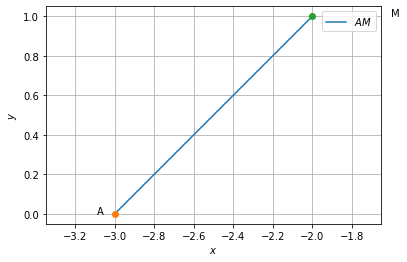
\includegraphics[width=\columnwidth]{solutions/su2021/2/14/de/Line_Plot_Part-1 (4).PNG}
\caption{Plot of Line $AB$ (Part-1)}
\label{linform/14/dePlot of Line $AB$ (Part-1)}
\end{figure}

\item Given point $\vec{A} = \myvec{0\\2}$.From the given information we have, $\tan30\degree =m = \frac{1}{\sqrt{3}}$.

The direction vector is $\vec{m} = \myvec{1\\\tan30\degree}$.  
Hence, the normal vector
\begin{align}
\label{linform/14/deeq:line_norm_dir2}
\vec{n} &= \myvec{0&-1\\1&0}\vec{m} 
\\
&= \myvec{-\tan30\degree\\1}
\end{align}
The equation of the line in terms of the normal vector is then obtained as
\begin{align}
\label{linform/14/deeq:line_norm_vec2}
\vec{n}^T\brak{\vec{x}-\vec{A}} &= 0
\\
\implies \myvec{-1 &\sqrt{3}}\vec{x} &=2{\sqrt{3}}
\end{align}
and plotted in Fig. \ref{linform/14/dePlot of Line $AB$ (Part-2)}.
\begin{figure}[ht]
\centering
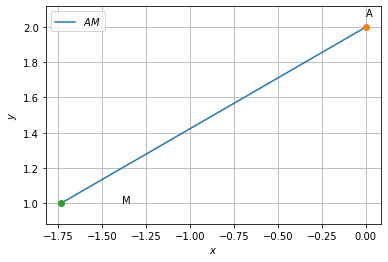
\includegraphics[width=\columnwidth]{solutions/su2021/2/14/de/Line_Plot_Part-2 (3).PNG}
\caption{Plot of Line $AB$ (Part-2)}
\label{linform/14/dePlot of Line $AB$ (Part-2)}
\end{figure}
\end{enumerate}
